\begin{myposter}{
    Глава 2. Результаты расчетов. Движения 1 и 2.
}

    \headerbox
    {Движение 1 ($\nu_{1,2}(0) = 0, \nu_3 = 1$)}
    {name=first,column=0,row=0,span=3}
    {
        {\huge\bf
            \vspace{10pt}
            \begin{figure}[H]
                \centering
                \minipage{0.3\textwidth}
                    \centering
                    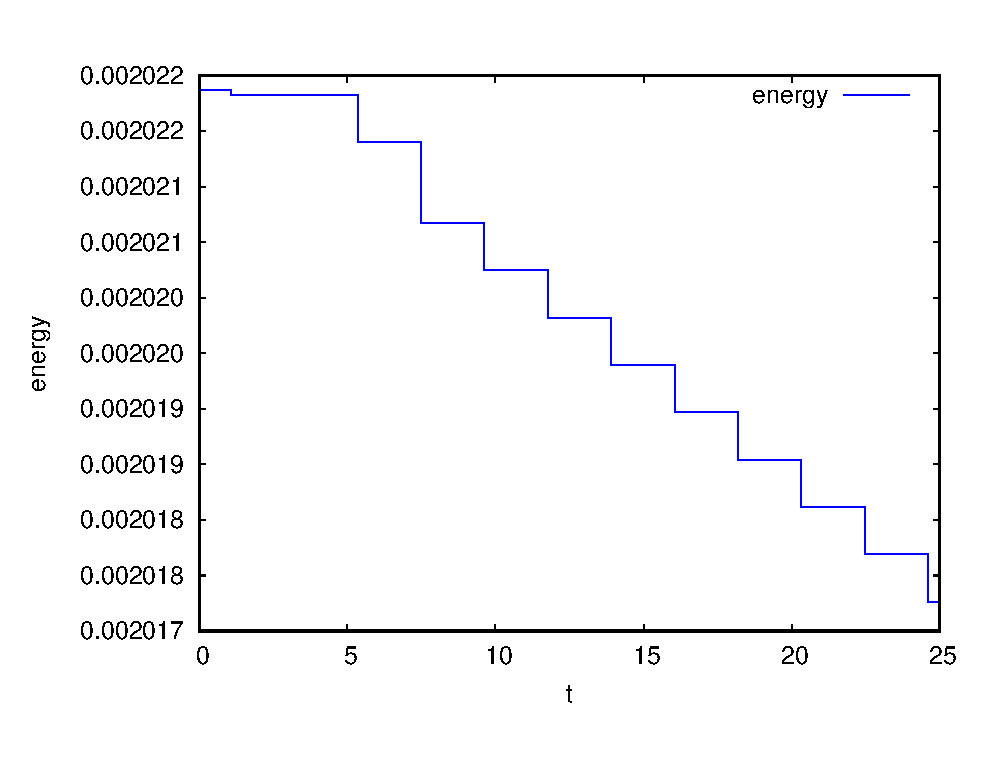
\includegraphics[width=\linewidth]{content/pic/self_rot_25/kin_en.eps}
                    \vspace{-15pt}
                    \caption{{\huge\bfКинетическая энергия $T$}}
                \endminipage
                \enspace
                \minipage{0.3\textwidth}
                    \centering
                    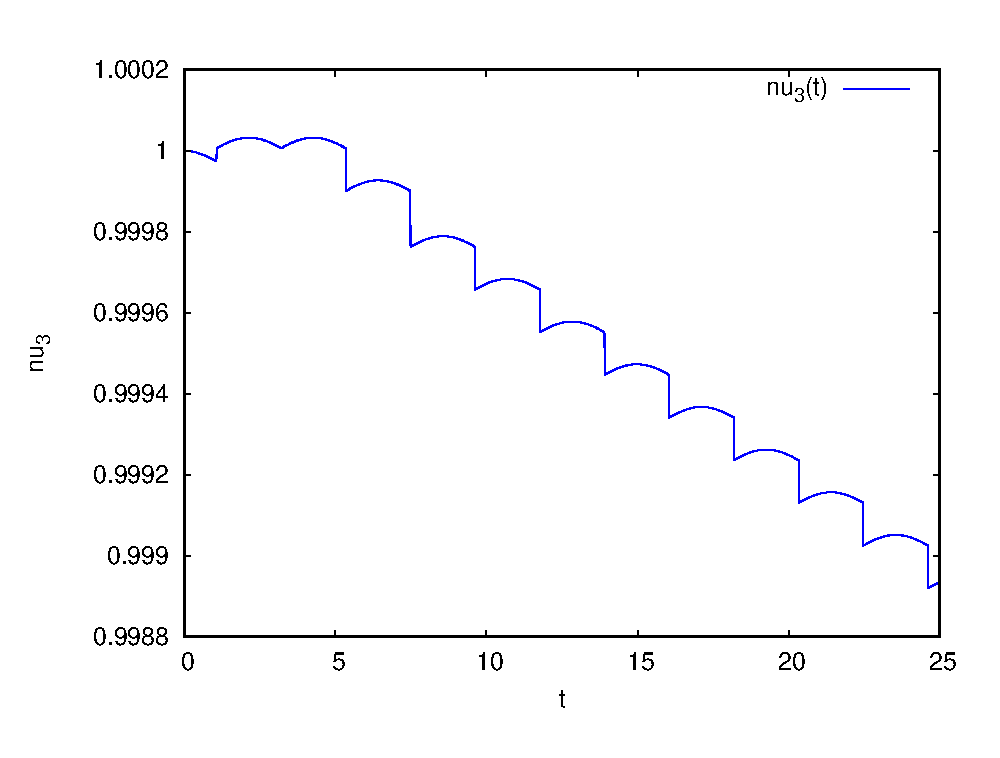
\includegraphics[width=\linewidth]{content/pic/self_rot_25/nu3.eps}
                    \vspace{-15pt}
                    \caption{{\huge\bfУгловая скорость $\nu_3$ платформы}}
                \endminipage
                \enspace
                \minipage{0.3\textwidth}
                    \centering
                    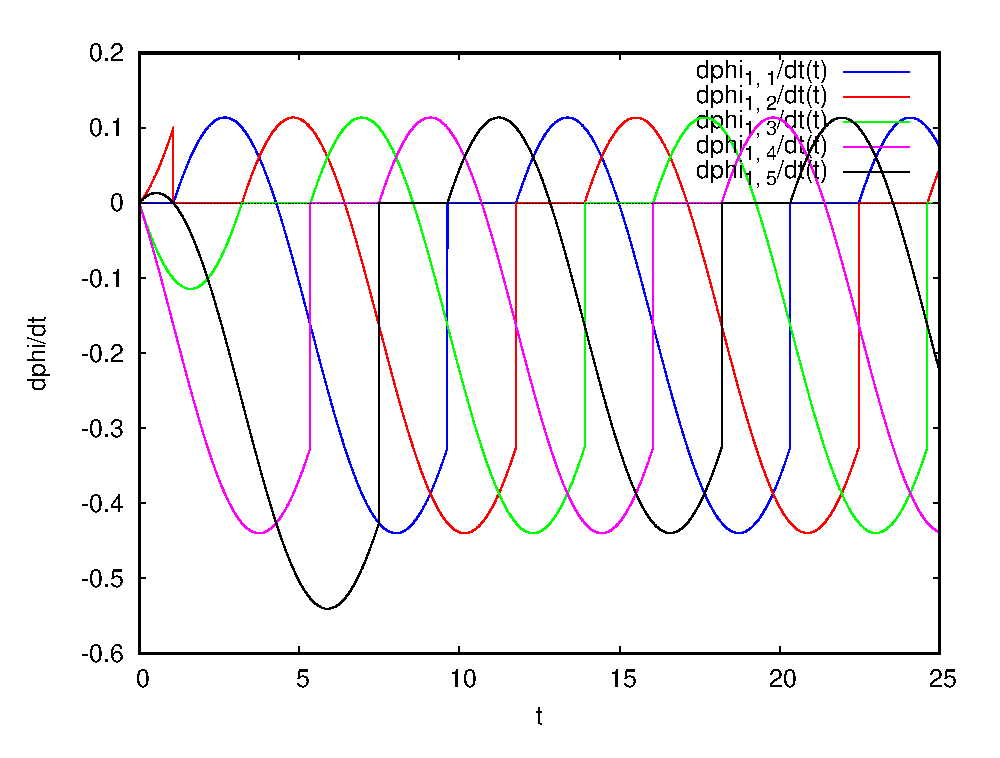
\includegraphics[width=\linewidth]{content/pic/self_rot_25/rol_vel.eps}
                    \vspace{-15pt}
                    \caption{{\huge\bfУгловые скорости роликов $\dot{\varphi}_{1\cdot}$}}
                \endminipage
            \end{figure}
            \vspace{10pt}
        }
    }
    
    \headerbox
    {Движение 2 ($\nu_1(0) = 1, \nu_{2,3} = 0$)}
    {name=second,column=0,row=1,below=first,span=3}
    {
        {\huge\bf
            \vspace{10pt}
            \centering
            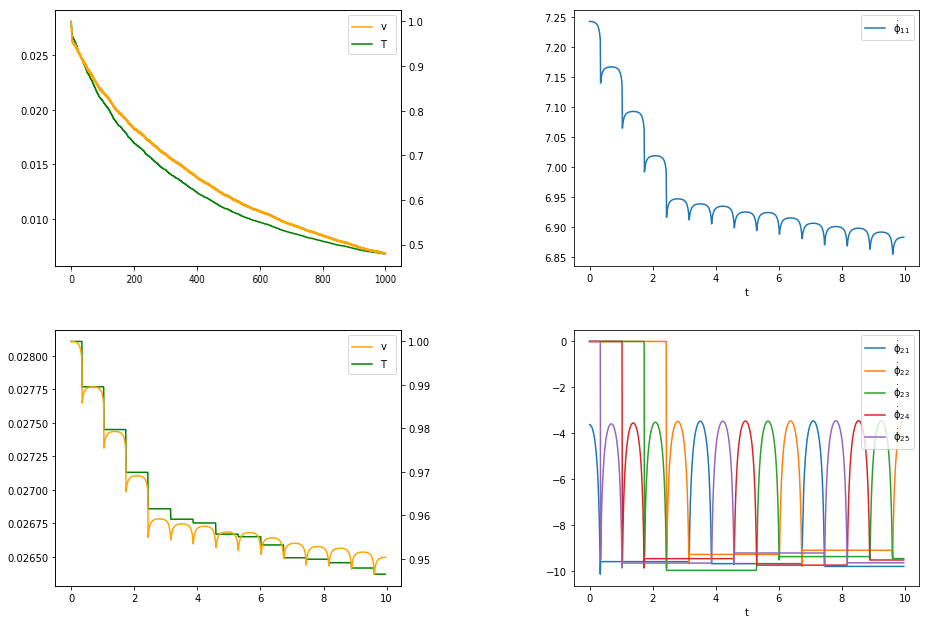
\includegraphics[width=\linewidth]{content/pic/new/impact_2_sub.png}
            \minipage{0.45\textwidth}
                \huge{Кинетическая энергия $T$ и скорость $v$ центра масс}
            \endminipage
            \qquad
            \minipage{0.45\textwidth}
                \huge{Угловые скорости роликов $\dot{\varphi}_{1\cdot}$}
            \endminipage
            \vspace{10pt}
        }
    }
    
\end{myposter}
